\chapter{Telemanipulátor jelfeldolgozó rendszere}
\label{sec:elektronika}

A bemutatott fizikai rendszerhez tartozó jelfeldolgozó rendszer hardveres elemei nem sokban térnek el a szakdolgozatomban használt megoldásoktól. Mégis jelentősen összetettebbé vált az elmúlt két évben azáltal, hogy mennyi mindent sajátítottam el a képzés végére. Kiegészítettem néhány biztonsági és jelminőséget javító funkcióval. Ebben a fejezetben igyekszem részletesen bemutatni a telemanipulátor aktuális pozíciójának meghatározására kiválasztott szenzorokat és a mikrovezérlőt.

%----------------------------------------------------------------------------
\section{Jelfeldolgozó rendszer koncepciója}

A komponensek bemutatása előtt a szögmérésre felépített rendszer elvét szeretném bemutatni. A rendszernek hasonlóan a fizikai vázhoz a tervezés során meghatározott elvárásoknak kell megfelelnie. Ugyan a \ref{sec:ujratervezesi_szempontok} fejezetben felsorolt elvárások száma lényegesen kisebb mint a vázzal vagy a programmal szemben támasztottak, viszont legalább annyira lényegesek. Komolyabb teljesítmény elektronikát nem kellett tervezzek a rendszerhez, mert a kiválasztott mikrovezérlő DC kimenete bőven képes előállítani a szenzorok feltáplálásához szükséges áramot. Amit viszont már a fizikai rendszer tervezésénél figyelembe kellett vennem, hogy a kábelezés ne legyen túl nehézkes, hogy a kommunikációban a szenzor-mikrovezérlő távolságból származó ellenállás ne okozzon problémát. A szenzorok tesztelésénél foglalkoztam a maximálisan használható drót hossz megállapításával. A rendszert a lehető legegyszerűbben, a lehető legkevesebb egyedi alkatrész felhasználásával készítettem el. A hangsúlyt a \ref{sec:mikrovez_bemut}.fejezetben bemutatásra kerülő mikrovezérlő kiválasztására fektettem. Nem volt szükség méret vagy egy fizikai korlát használatára, így igyekeztem a lehető legnagyobb teljesítményű és legtöbb potenciális továbbfejlesztést lehetővé tévő megoldást választani. A következőkben a már megépített rendszert és a lehetséges továbbfejlesztési lehetőségeket bemutatni.

\begin{figure}[!ht]
\centering
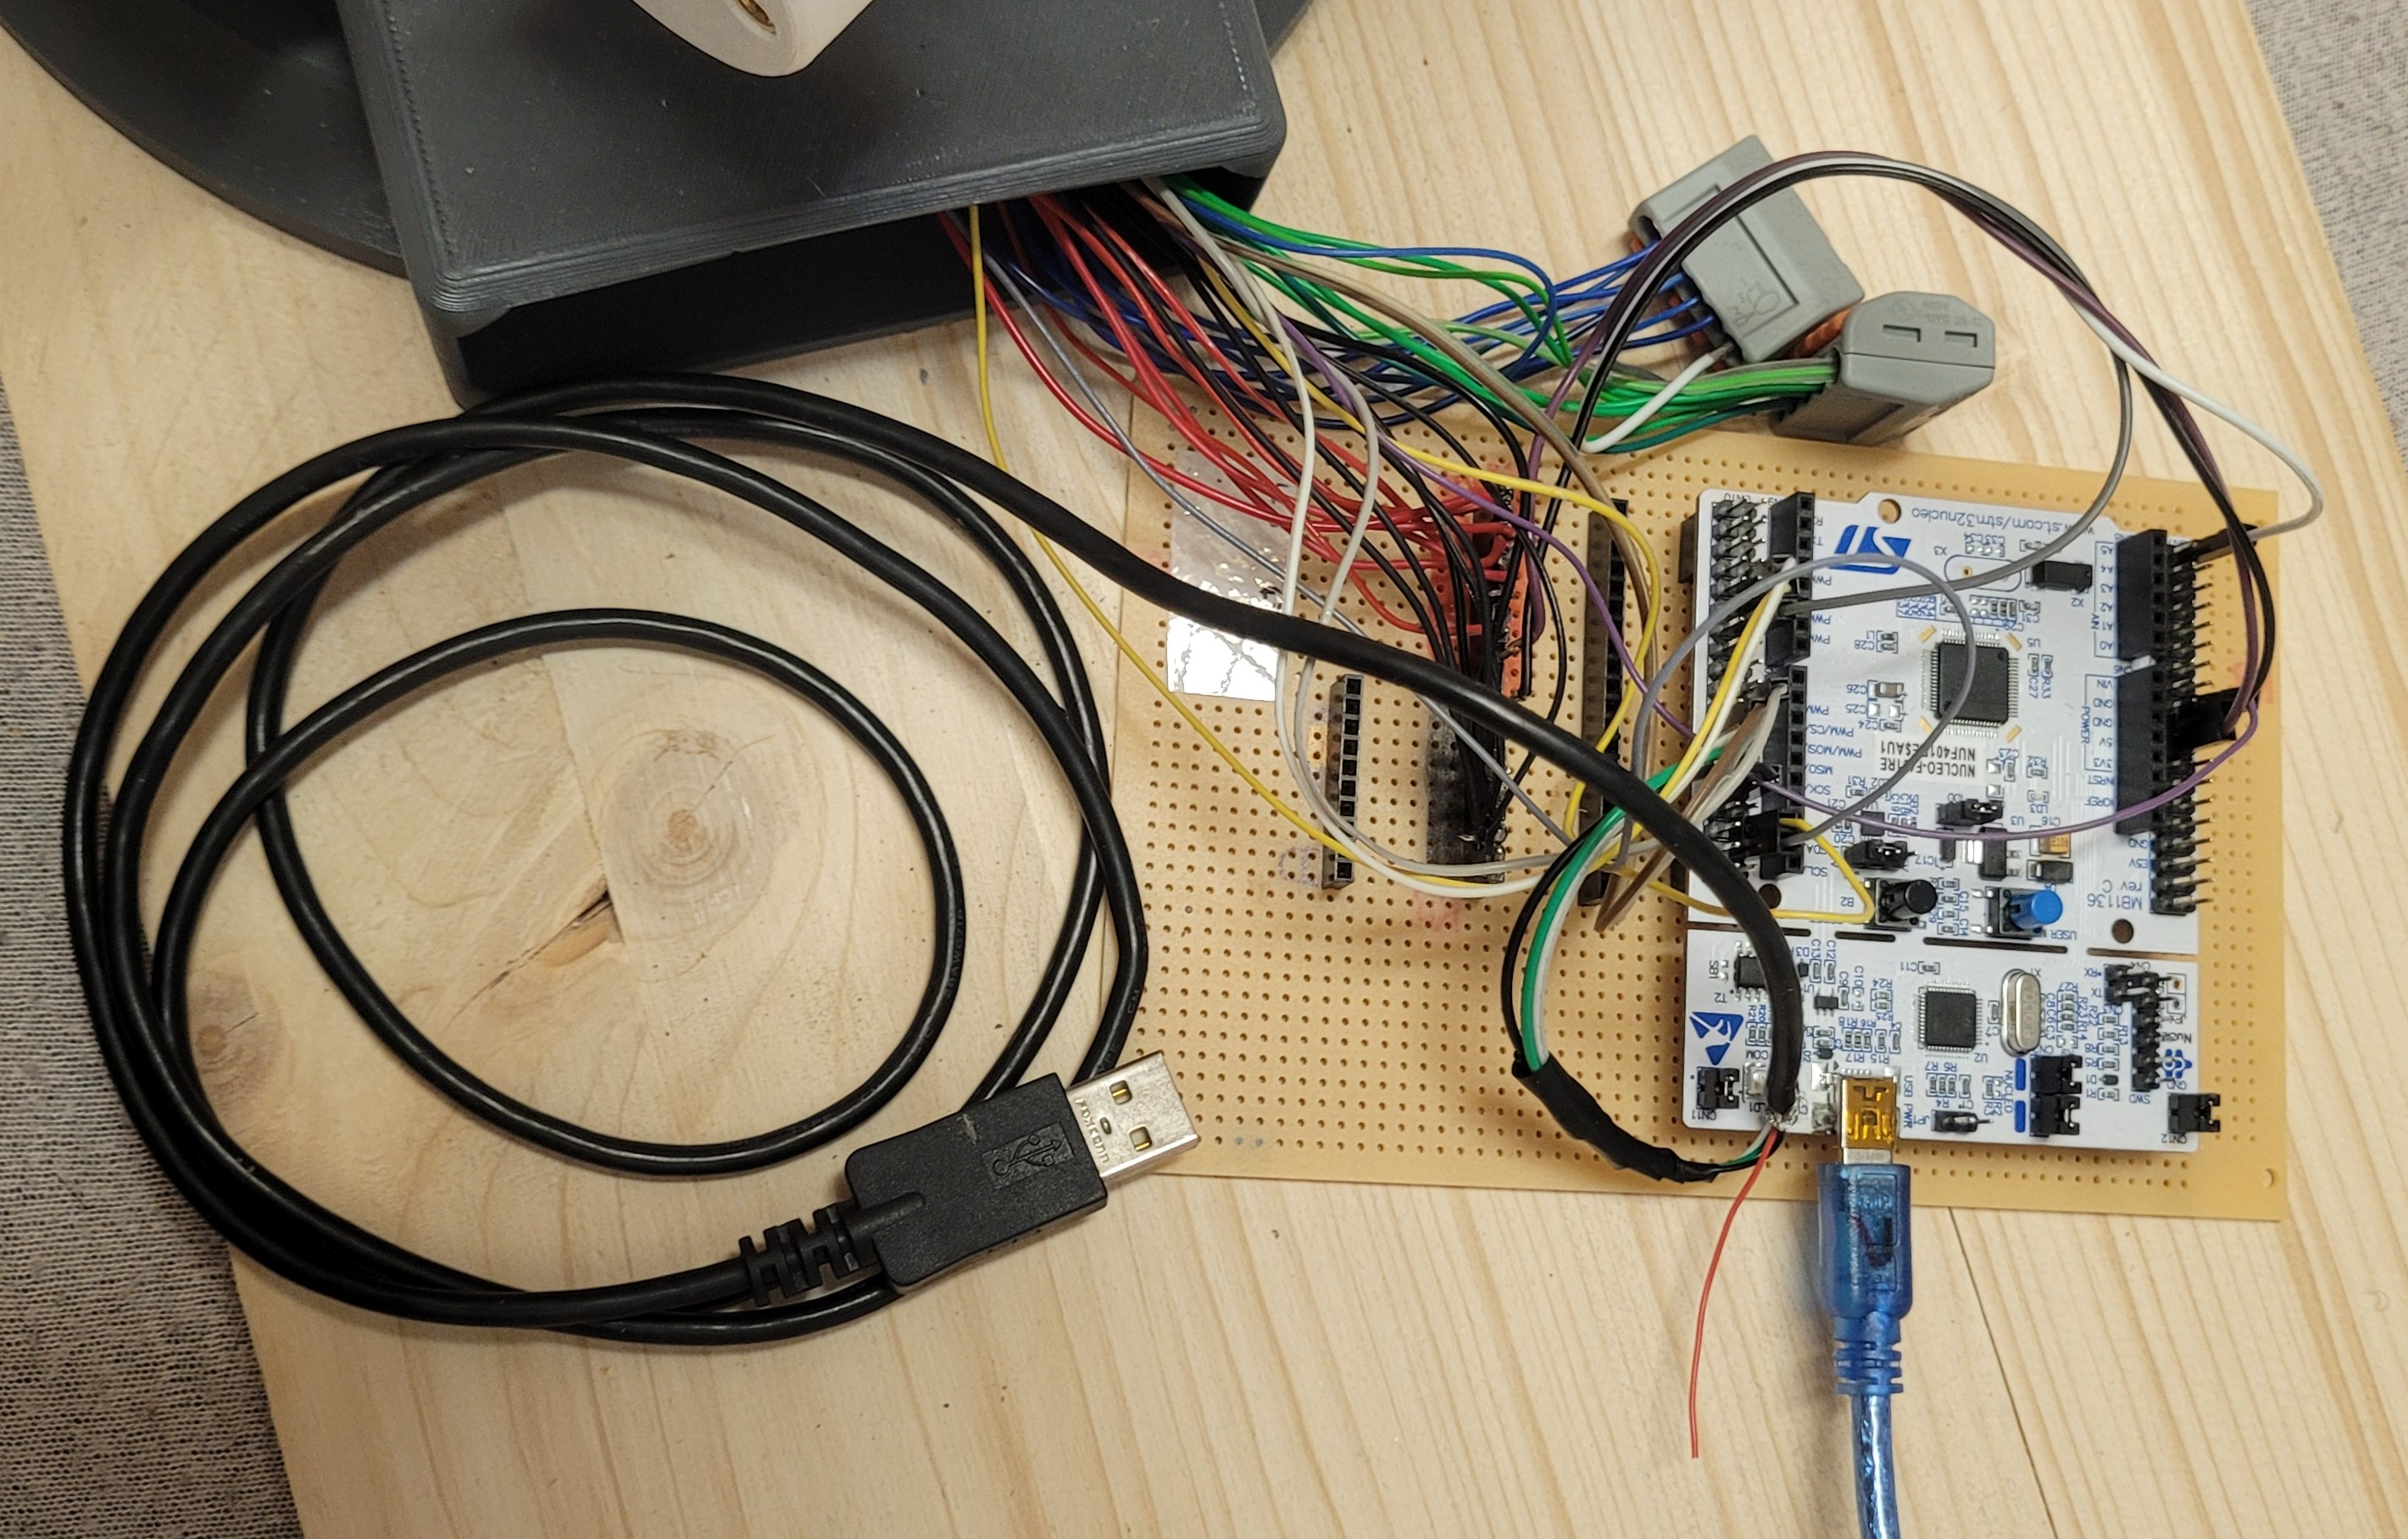
\includegraphics[width=100mm, keepaspectratio]{figures/Csuklo_szog_teszt/mikrovez_2}
\caption{Az elkészült jelfeldolgozó rendszer}
\label{fig:mikrovez_2}
\end{figure}

%----------------------------------------------------------------------------
\section{Jelfeldolgozó rendszer összeállítása}

A jelfeldolgozó rendszer elektronikai oldalról minimális mérnöki ismeretekkel is könnyen megérhető és a bemutatása is igen egyszerű. Az összeállítást a csuklóban érzékelt szögtől indulva mutatom be lépésről-lépésre. Egy adott csuklóból induló két kar egymással bezárt szögének mérésére GMR(Giant magnetoresistance) szenzort használtam. A szenzor működését \ref{sec:gmr_leiras}.fejezetben részletesen bemutatom. A szenzor összeállítás magából a szenzorból és a szenzorlapjával párhuzamba állított mágnesből áll. Ezzel a szenzor összeállítással a jeladó és a jelvevő között fizikai kontaktus nélkül tudok szöget mérni. Viszont ami még lényegesebb nincs végállása a szenzornak. Így a váz tervezése során csak azt kellett figyelembe vennem, hogy a szenzor és a mágnes középtengelye egybe essen és a távolságuk ne legyen nagyobb mint $17[mm]$. A szenzorhoz saját magam által tervezett és gyártott NyÁK lapot használtam, mivel a szenzor SMD\footnote{ Surface Mount Device rövidítése, magyarul felszíni szerelésű eszköz. Az SMD elektronikai elemek olyan alkatrészek, amelyek kis méretűek és a nyomtatott áramköri lap felszínére vannak forrasztva.} kivitelű, ezért szükséges volt megoldani a szenzor chip lábai és a drót közötti kapcsolatot.

\begin{figure}[!ht]
\centering
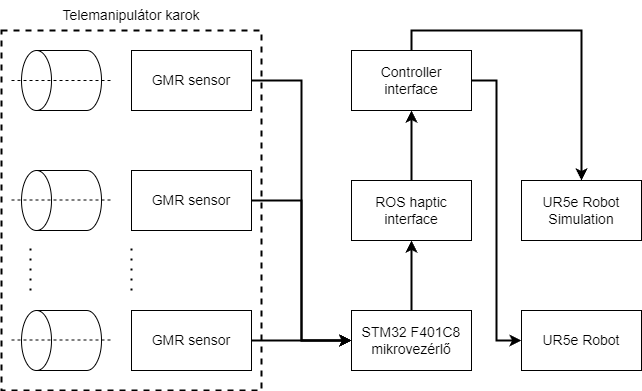
\includegraphics[width=125mm, keepaspectratio]{figures/Diagrammok/Telemanipulator_teljesrendszer}
\caption{A jelfeldolgozó rendszert szemléltető ábra}
\label{fig:Telemanipulator_teljesrendszer}
\end{figure}

A következő fontos komponens a bypass kondenzátor. Ennek a kondenzátornak a célja a teljesítmény ingadozás kiküszöbölése, ezzel a szenzor működése egyenletesebbé tehető. Ezt a javaslatot a bypass kondenzátor használatára még a szakdolgozatom bírálatánál kaptam, mint lehetséges teljesítmény javító komponens.

Tovább folytatva a bemutatást, részletesebben szeretném bemutatni a drótok csatlakozóit, ugyanis a szakdolgozatban elkészített telemanipulátor szenzoraihoz tartozó drótok nem voltak megbonthatóak az összeállítás teljes hosszában. Ez a későbbi továbbfejlesztési lehetőséget akadályozta meg. Ebben a dolgozatban bemutatott eszköznél már a váz fizikai paramétereinek megadásánál figyeltem, hogy csatlakozókat tudjak a szenzoroknál elhelyezni. A végső változatban a szenzor után $30-40[mm]$-re helyeztem el minden bontó csatlakozót, hogy a tengelyeket a mozgásban ne akadályozza, de bármilyen probléma esetén könnyen hozzáférhető legyen. Ez az extra elem a későbbiekben a leghasznosabb fejlesztésnek bizonyult, ugyanis a szenzorok üzembe helyezése alatt a hiba keresést leegyszerűsítette, hogy nem kellett a mikrovezérlő bekötéseit megbontanom ahhoz, hogy külön leellenőrizhessem a működést.

A megfelelő drót kiválasztás a nem kritikus, de érdemes odafigyelni. Két hardver szempontjából lényeges kritériumot fogalmaztam meg és két szerelési kritériumot támasztottam ezzel szemben. Ezek a következőek voltak:

\begin{itemize}
  \item A drótnak a minimális fordulási sugarának alacsonynak kell lennie. Ez azért fontos, mert a szakdolgozatnál készített manipulátor esetében ezt nem vettem figyelembe és a drótok a használat közbeni deformációja nehezítették a mozgatást
  \item A drót egységnyi hosszon mért ellenállása ne akadályozza a szenzorok működését. Ez kevésbé fenyegető probléma, azonban érdemesnek tartottam figyelembe venni, ugyanis a hatodik szenzor és a mikrovezérlő távolsága megközelíti $1000[mm]$-t. Ez a későbbiekben bekövetkező tovább fejlesztést akadályozhatja meg.
  \item Szerelési kritériumként figyelembe vettem a drótok maximális átmérőjét. Több esetben 2-3 szenzorhoz tartozó kábelezés lép át egy adott csuklóban egyik karban futó csatornából a másikba. A probléma leküzdését két oldalról közelítettem meg. Egyrészt a maximális drót számhoz tartozó átmérőnek a $400[\%]$-át vettem minimum keresztmetszetnek minden csuklóban. Másodsorban szignifikánsan nagyobb csapágyakat választottam mint a szakdolgozatomban, így gyakorlatilag akár 20-30 szenzor elvezetése is lehetséges lenne a csukló tengelyeknél.
  \item A szerelés megkönnyítésére nagyon fontos és az egyszerű hibakeresésnél lényeges, hogy minden szenzorhoz tartozó a szenzorválasztójelét továbbító drót jól megkülönböztethető legyen. Röviden megfogalmazva a drótból, amit választok legalább $11$ féle szín legyen elérhető. Ez a gond a szakdolgozatban épített telemanipulátor újra indításánál jelentkezett. Rengeteg időt vett el a szenzorok újra beazonosítása.
\end{itemize}

Ezek a meghatározott kritériumok egy része kényelmi és inkább magasabb bekerülési költséget eredményeznek, de a teljes rendszer finanszírozhatóságával később szeretnék foglalkozni.

A következő komponensek már lényegesen összetettebbek. Logikai sorrendben a mikrovezérlő(MCU\footnote{Micro Controller Unit - magyarul mikrovezérlő}) következik. Az MCU végzi a szenzorok áramellátását, velük való kommunikációt, az adatok feldolgozását és ezek továbbítását. Az MCU program leírását a \ref{sec:MCU_program}.fejezetben részletesebben is megteszem. A mikrovezérlő USB kommunikációs porton csatlakozik a számítógépre, míg a saját bootloaderével\footnote{A bootloader egy speciális szoftver, amely lehetővé teszi az alkalmazásfirmware frissítését vagy telepítését a mikrovezérlőn keresztül.} a program felügyeletét lehet végezni.

%----------------------------------------------------------------------------
\section{Elektronikai rendszer komponensei}

A komponensek kiválasztása egyes esetekben más és más szempontok alapján történik. Az egyik oka, hogy költségelemezést végeztem a telemanipulátorral kapcsolatban a dolgozatom végén (XYZ fejezet), hogy egy átfogó képet készítsek arról, hogy jelenleg egy ilyen végletekig leegyszerűsített prototípus körülbelül mekkora előállítási költséggel jár. A komponensek kiválasztási szempontjaiban az elérhetőséget és a későbbi továbbfejleszthetőséget tartottam szem előtt. Az alkatrészek bemutatásánál nem térek ki a szerelvények minden elemére, mert például az USB kábel legoptimálisabb kiválasztására nem fektettem energiát. Csakúgy mint a rendszer koncepciós bemutatásánál szenzortól haladva a nagyobb egységekig fogom bemutatni az elemeket részletesebben.

%----------------------------------------------------------------------------
\subsubsection{GMR szenzor}
\label{sec:gmr_leiras}

A csukló szög megállapításához használt szenzor összeállításban a korongmágnes állását mértem egy mágneses térorientációt mérni képes szenzorral. A Giant Magnetoresistance (GMR) egy olyan érzékelő, amely az szenzorban található ellenállások elektromágneses tulajdonságaiknak változását méri egy mágneses mező hatására. Ez a technológia a mágneses rezisztivitás változását használja ki, amikor egy mágneses tér hatására az elemben levő részecskék mágneses állapota változik. A szenzor működése röviden úgy foglalható össze, hogy a szenzorok több réteg vékony filmrétegből állnak, amelyek között ferromágneses és nem-ferromágneses rétegek váltakoznak. A ferromágneses rétegek mágneses polarizációjukat megváltoztathatják a külső mágneses tér hatására, és ezáltal befolyásolják az elektromos ellenállást az érzékelőben. Ennek a változásnak a szenzorba mérőrendszer képes a mágneses pólusok orientációját megadni a szenzor tengelyeihez képest.

\begin{figure}[!ht]
\centering
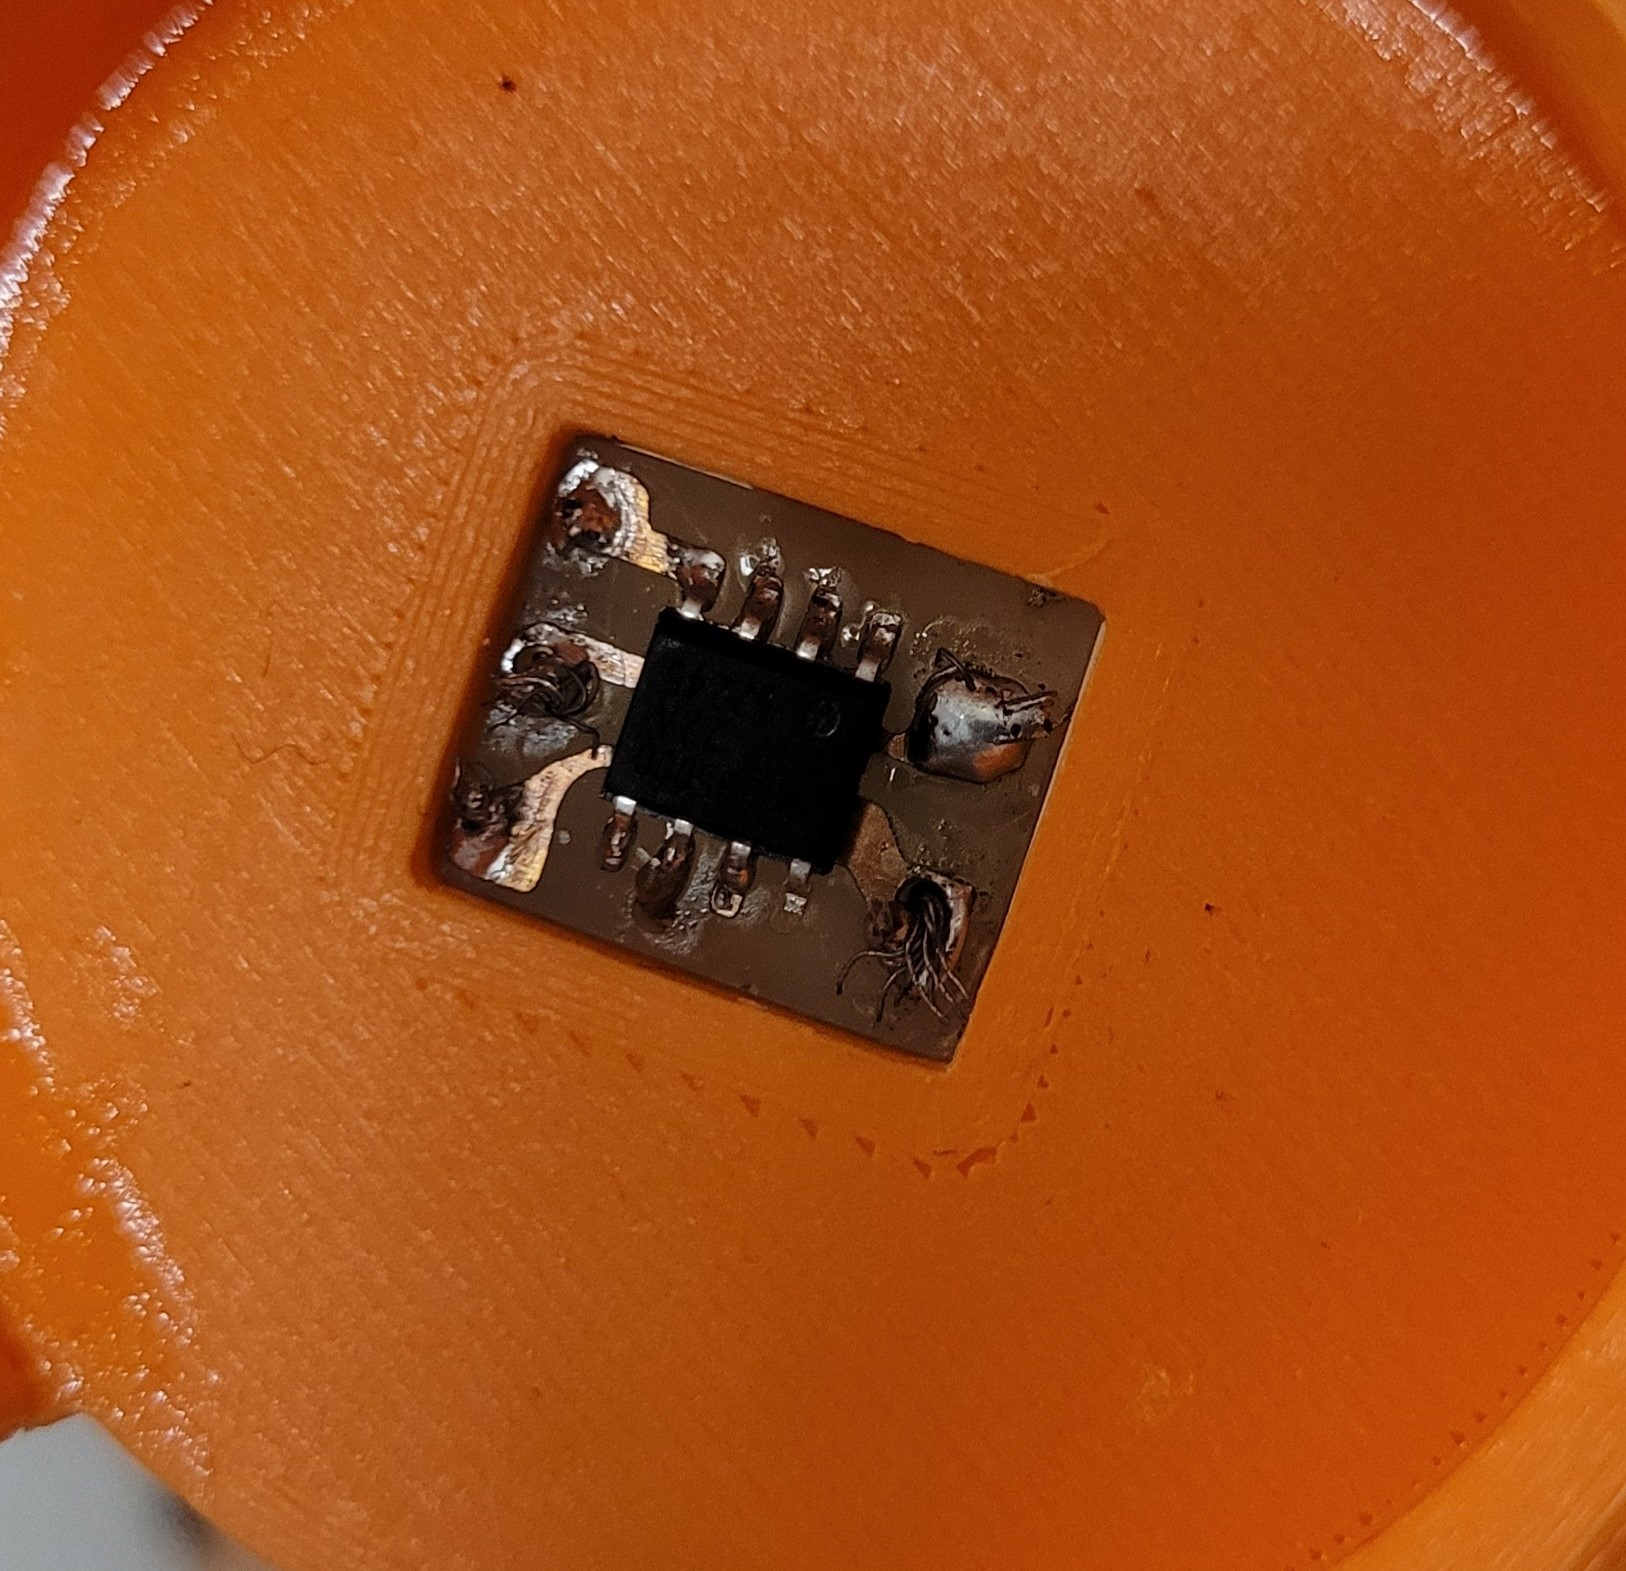
\includegraphics[width=65mm, keepaspectratio]{figures/Csuklo_szog_teszt/szenzor}
\caption{A NyÁK lapra helyezett GMR szenzor}
\label{fig:csuklo_szenzor_pcb}
\end{figure}

Az általam használt szenzor az Infineon TLE5012B jelzésű GMR szenzor. Ez a szenzor egy $360[^\circ]$-os szögérzékelő. Ezt az érzékelést monolitikusan integrált\footnote{A monolitikus integrált áramkörben az áramkör valamennyi aktív és passzív elemét, valamint a hozzájuk tartozó összekötéseket egyetlen chip-ben alakítják ki. Ezt a kialakítást szokás félvezető alapú integrált áramkörnek is nevezni.} Giant Magneto Resistance (GMR) elemekkel mérik, melyek a szinusz és koszinusz szögkomponenseit érzékelik a mágneses pólusoknak. Ezeket a nyers jeleket belsőleg digitálisan feldolgozzák a mágneses tér orientációjának kiszámításához. Ami nagyon fontos, hogy ez az érzékelő egy előre-kalibrált érzékelő. A kalibrációs paramétereket belsőleg tárolják. A bekapcsoláskor ezekhez viszonyítva adja meg a szögértékeket a szenzor. A szögmérés pontosságát egy opcionális belső automatikus kalibrációs algoritmussal lehet javítani a hőmérséklettartomány  és élettartam függvényében. Én ezt a funkciót nem használtam, de a mikrovezérlő programjába integráltam ennek a lehetőségét, de erről majd a \ref{sec:Prog_nagy_fej}.fejezetben a szenzor programozása kapcsán említést teszek. Az adatkommunikációt egy kétirányú Szinkron Soros Kommunikációval\footnote{A \ref{sec:ssc_kom}.fejezetben részletesen bemuatatom} (SSC) valósítják meg, amely SPI-kompatibilis. Utóbbi azért fontos, mert legelterjedtebben a SPI protokoll elérhető a mikrovezérlőknél. A szenzor konfigurációja regiszterekben tárolódik, amelyek elérhetők az SSC interfésszel. Emellett négy másik interfész is rendelkezésre áll a TLE5012B-vel: Impulzus-Szélesség-Moduláció (PWM) Protokoll, Rövid PWM Kód (SPC) Protokoll, Hall Kapcsoló Mód (HSM) és Inkrementális Interfész (IIF). Ezeket az interfészeket az SSC-vel együtt vagy önállóan lehet használni. Előre konfigurált érzékelő változatok elérhetők különböző interfészbeállításokkal, de a telemanipulátornál én, csak a SSC kommunikációs megvalósítást használtam. Ez a legegyszerűbb és az általam használt program könyvtár is erre volt optimalizálva. Néhány fontosabb jellemzőt még felsorolok a szenzorról, amik fontosabbak:

\begin{itemize}
	\item Egy chipben van minden. Nincs szükség további komponensre a szenzor működtetéséhez.( A bypass kondenzátor is inkább csak pontosság és megbízhatóság javító kiegészítő )
	\item $360[^\circ]$-os szögmérés fordulatszámlálóval és szögsebesség méréssel. Ugyan nem használom ki szögsebesség mérést, de mint lehetőség későbbiekben a gravitációs hatásából származó terhelés kikompenzálásában még szerepe lehet. A $360[^\circ]$-os mérés pedig külön előny, hogy nem kell foglalkozni az összeszerelésnél az orientációval, offszeteléssel be lehet könnyedén állítani.
	\item 15 bites szögérték megadás a kimeneten, aminek pontossága $0,01[^\circ]$. Ez kellően nagy felbontás ahhoz, hogy a telemanipulátor end-effektorának pozícióját meghatározzam
	\item 16 bit-en értelmezett szinusz / coszinusz érték az interfészen
	\item Maximum $1[^\circ]$ hiba a gyártó által garantálva, szenzor élettartalma és környezeti hőmérséklet függvényében
	\item Két irányú SSC kommunikációs protokol az interfészen, ami $8[\frac{Mbit}{s}]$-ig emelhető. A szenzor mérés szögmérésének periódus ideje minim $0,001366[ms]$, ami bőven a $4[ms]$-os cél érték alatt van.
	\item Számos egyéb kommunikációs protokoll \textbf{SSC}, PWM, IIF, HSM, SPC
	\item A chip választó pin többféleképpen konfigurálható. (push-pull vagy open-drain)
 	\item Magas hőmérséklet tűréshatár: $-40[^\circ C]-tól~150[^\circ C]-ig$
	\item Nem tartalmaz halogént
\end{itemize}

\begin{figure}[!ht]
\centering
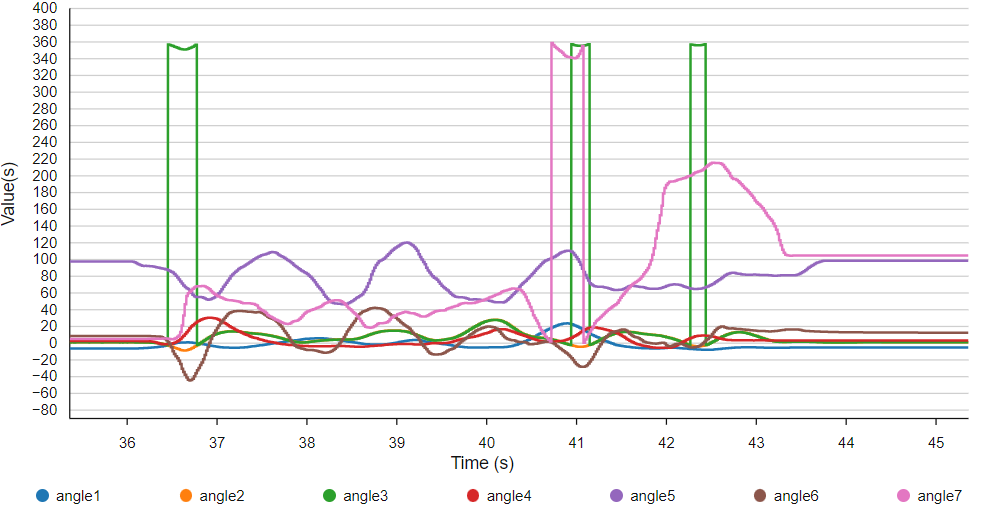
\includegraphics[width=100mm, keepaspectratio]{figures/Csuklo_szog_teszt/szumma}
\caption{Az csuklóban található szenzorok működés közben}
\label{fig:csuklo_teszt_szumma}
\end{figure}

Ez a szenzor kellő megbízhatóságú a tapasztalataim alapján, kézi forrasztás közben jól kezelhető és nem érzékeny a magas forrasztási hőmérsékletre. Kifejezetten pontos és rendkívül gyors számítással rendelkezik ezért ideális a telemanipulátorhoz tartozó karok szögértékének mérésére. A dolgozatomban még kitérek a szenzorok tesztelésére.

%----------------------------------------------------------------------------
\subsection{Bypass kondenzátor}

A szakdolgozatom bírálásában kaptam javaslatként, hogy egészítsem ki a szenzor NyÁK-ot egy bypass kondenzátorral. A képzésem további szakaszában részletesebben tanultunk is erről a típusú alkalmazási lehetőségről a kondenzátorok esetében. A bypass kondenzátorok olyan elektromos komponensek, amelyeket általában abból a célból alkalmaznak, hogy a stabilitást, zajszűrést és teljesítményjavulást érjenek el. Ezek a kondenzátorok képesek "bypass"-olni, azaz át vagy elvezetni az áramot bizonyos alkatrészek mellett. Kicsit részletesebben bemutatnám a kondenzátor működését és azt, hogy mely jellemzőket kihasználva lehet ezt a bypassoló hatást elérni. A kondenzátorok alapvetően két vezető lemez között elhelyezkedő dielektromos anyagból állnak. Amikor az elektromos feszültség megváltozik, a kondenzátorban tárolt elektromos töltés is változik. Ennek eredményeként a kondenzátor karakterisztika függvényében felhalmozza majd átengedi az áramot. Ha ez periodikusan megtörténik, akkor a kondenzátor bizonyos frekvenciákon, akár a zajt vagy pusztán teljesítmény stabilitást adhat a rendszernek. Utóbbi jelenséget használjuk ki bypass kondenzátor esetében. Ezt a kondenzátor használati módot gyakran alkalmaznak a következőkbe felsorolt esetekben:

\begin{itemize}
	\item Zajszűrésre, különösen érzékeny elektronikai eszközök, például erősítők vagy analóg- digitális átalakítók környezetében. Ezek a kondenzátorok képesek alacsony frekvenciájú zajokat szűrni, javítva ezzel a jelerősséget.
	\item Stabilitás javítására, például mikroprocesszorok vagy más integrált áramkörök esetében a kondenzátorok segítenek kiegyenlíteni a feszültség-ingadozásokat.
\end{itemize}


\begin{figure}[!ht]
\centering
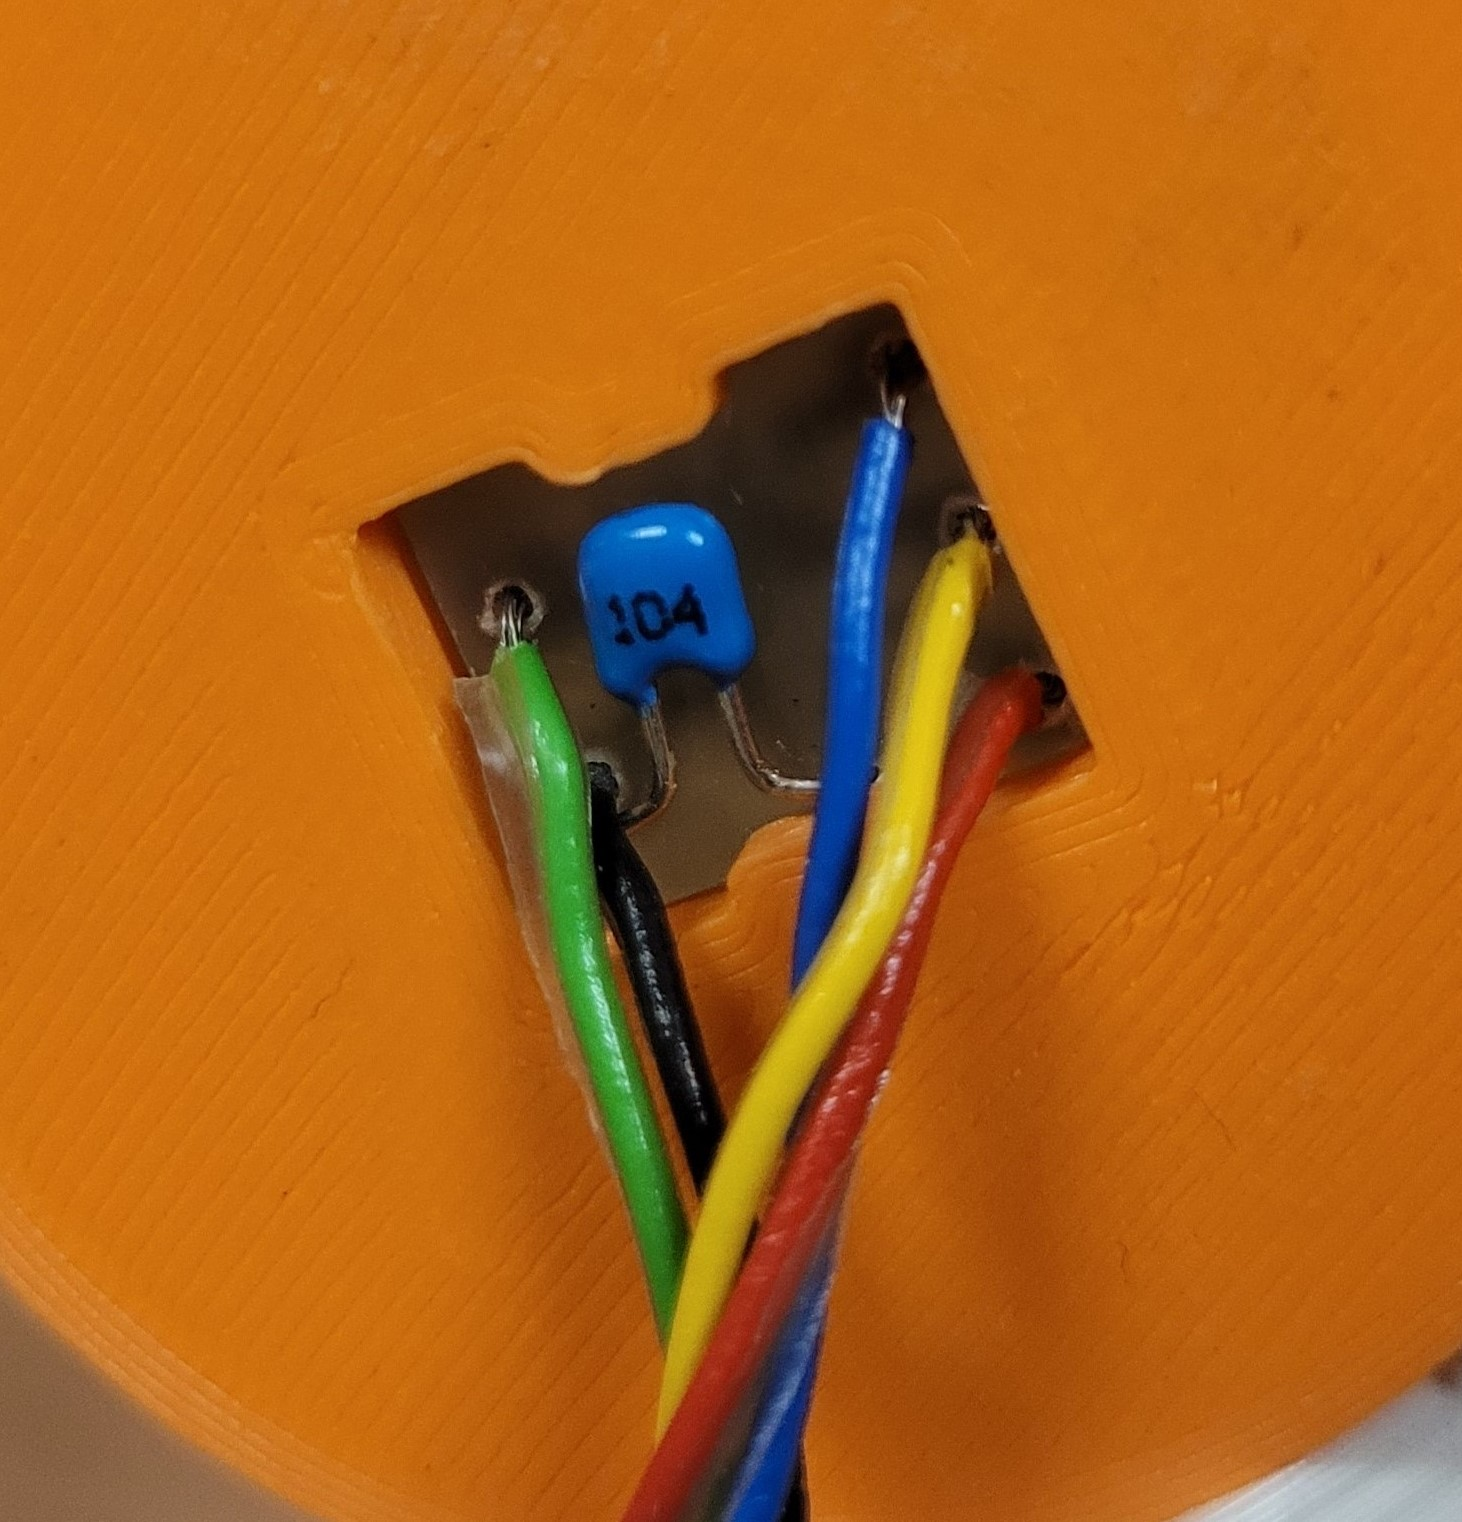
\includegraphics[width=70mm, keepaspectratio]{figures/Csuklo_szog_teszt/bypass}
\caption{A szenzoron található bypass kondenzátor beépítve}
\label{fig:bypass}
\end{figure}

A bypass kondenzátor elhelyezése kritikus a hatékony zajszűrés és kellő stabilitás szempontjából. A kondenzátort a szenzort tápláló lábak közvetlen közelébe kell elhelyezni. A képen is jól látható módon én a szenzor $3V3$-as lábának helye mellett helyeztem el a furatot, ennél közelebb nem-igen tudtam volna fúrni rögzítőfuratot. A $GND$ azaz föld a kondenzátor másik lába esetében annyira már nem fontos.

A megfelelő bypass kondenzátor kiválasztása fontos a kívánt teljesítmény eléréséhez. A kondenzátor értéke és típusa is nagymértékben befolyásolja a hatékonyságot. Az általam választott kondenzátor $100[nF]$-os $50-[V]$-os nyitó feszültséggel rendelkező kerámia kondenzátor. Az ilyen típusú kondenzátorok kiválóan teljesítenek magas frekvenciás alkalmazásokban, amelyekhez gyakran használják őket bypass kondenzátorként. Rendkívül jól használhatóak stabilitás és zajszűrés céljából. Kis méretűek és alacsony induktanciájúak, ami különösen fontos, mivel a szenzor kompakt és nem igen kiegészíthető más elemmel a zavaró jelek kiszűrése érdekében. Ezek mellett a kerámia kondenzátorok elérhetők különböző kapacitásértékekkel míg a méretük meglehetősen kicsi, így jól használhatóak kis méretű szenzorok esetében is, amilyenre nekem is szükségem van. A későbbiekben is ki fogok rá térni, de ezek a kondenzátorok általában gazdaságosak, ez hozzájárul a bekerülési költségek csökkentéséhez.

A kondenzátornak a paraméterei bőven túlméretezettek\footnote{Ennek a nyitó feszültség értéknek a fele is elegendő lenne a rendszer stabilitásának biztosítása érdekében}, mérete kellőképpen kicsi, olcsó és majdnem minden kiskereskedelmi egységben beszerezhető.

%----------------------------------------------------------------------------
\subsection{Csatlakozók}

Korábban említettem és a kritériumok közt is szerepelt, hogy minél flexibilisebbre szerettem volna a rendszert megtervezni. Ennek céljából külön odafigyeltem a csatlakozókra, hogy milyet használjak. A legkézenfekvőbbnek a MOLEX gyártó által elérhető csatlakozók bizonyultak. Ezek széles körben használt elektromos csatlakozók, és számos előnyt kínálnak, amelyek miatt népszerűek az elektronikai és ipari alkalmazásokban. Legnagyobb előnye, hogy a csatlakozók moduláris kialakításúak, ami lehetővé teszi, hogy kialakíthassunk velük egyszerű vagy összetett csatlakozási rendszereket az adott alkalmazáshoz. Ez a típus gyorsan és könnyen csatlakoztatható és bontható. Ez gyors telepítést és karbantartást tesz lehetővé, ami különösen előnyös összeszerelési, hibakeresési vagy fejlesztési esetekben. Széles körben alkalmazhatók különböző területeken, ennek eredményeként viszonylag egyszerű beszerezni. A Molex a minőségi termékeiről ismert, és csatlakozói megfelelnek a szigorú minőségi szabványoknak, ennek eredményeként a csatlakozók megbízhatóak és hosszú élettartamúak. Átfogó termékválasztékkal rendelkezik, beleértve különböző típusú csatlakozókat, vezetékeket, illetve kiegészítő termékeket. A telemanipulátor esetében 6 pin-es csatlakozókat választottam azért, hogy minden szenzornak saját vezeték párjai legyenek. Ezek a csatlakozók magas teljesítményű és nagy sebességű adatátvitelre alkalmasak, ami fontos volt a eszköz szempontjából. Ezeken felül a csatlakozók kis eséllyel kontaktosak\footnote{Rövid pillanatszerű vagy mozgásra vagy rezgésre megjelenő folytonosság hiba}, illetve az élettartalom se utolsó, mivel ezt a rendszer a lehető leggazdaságosabban a legtovább működteti.

\begin{figure}[!ht]
\centering
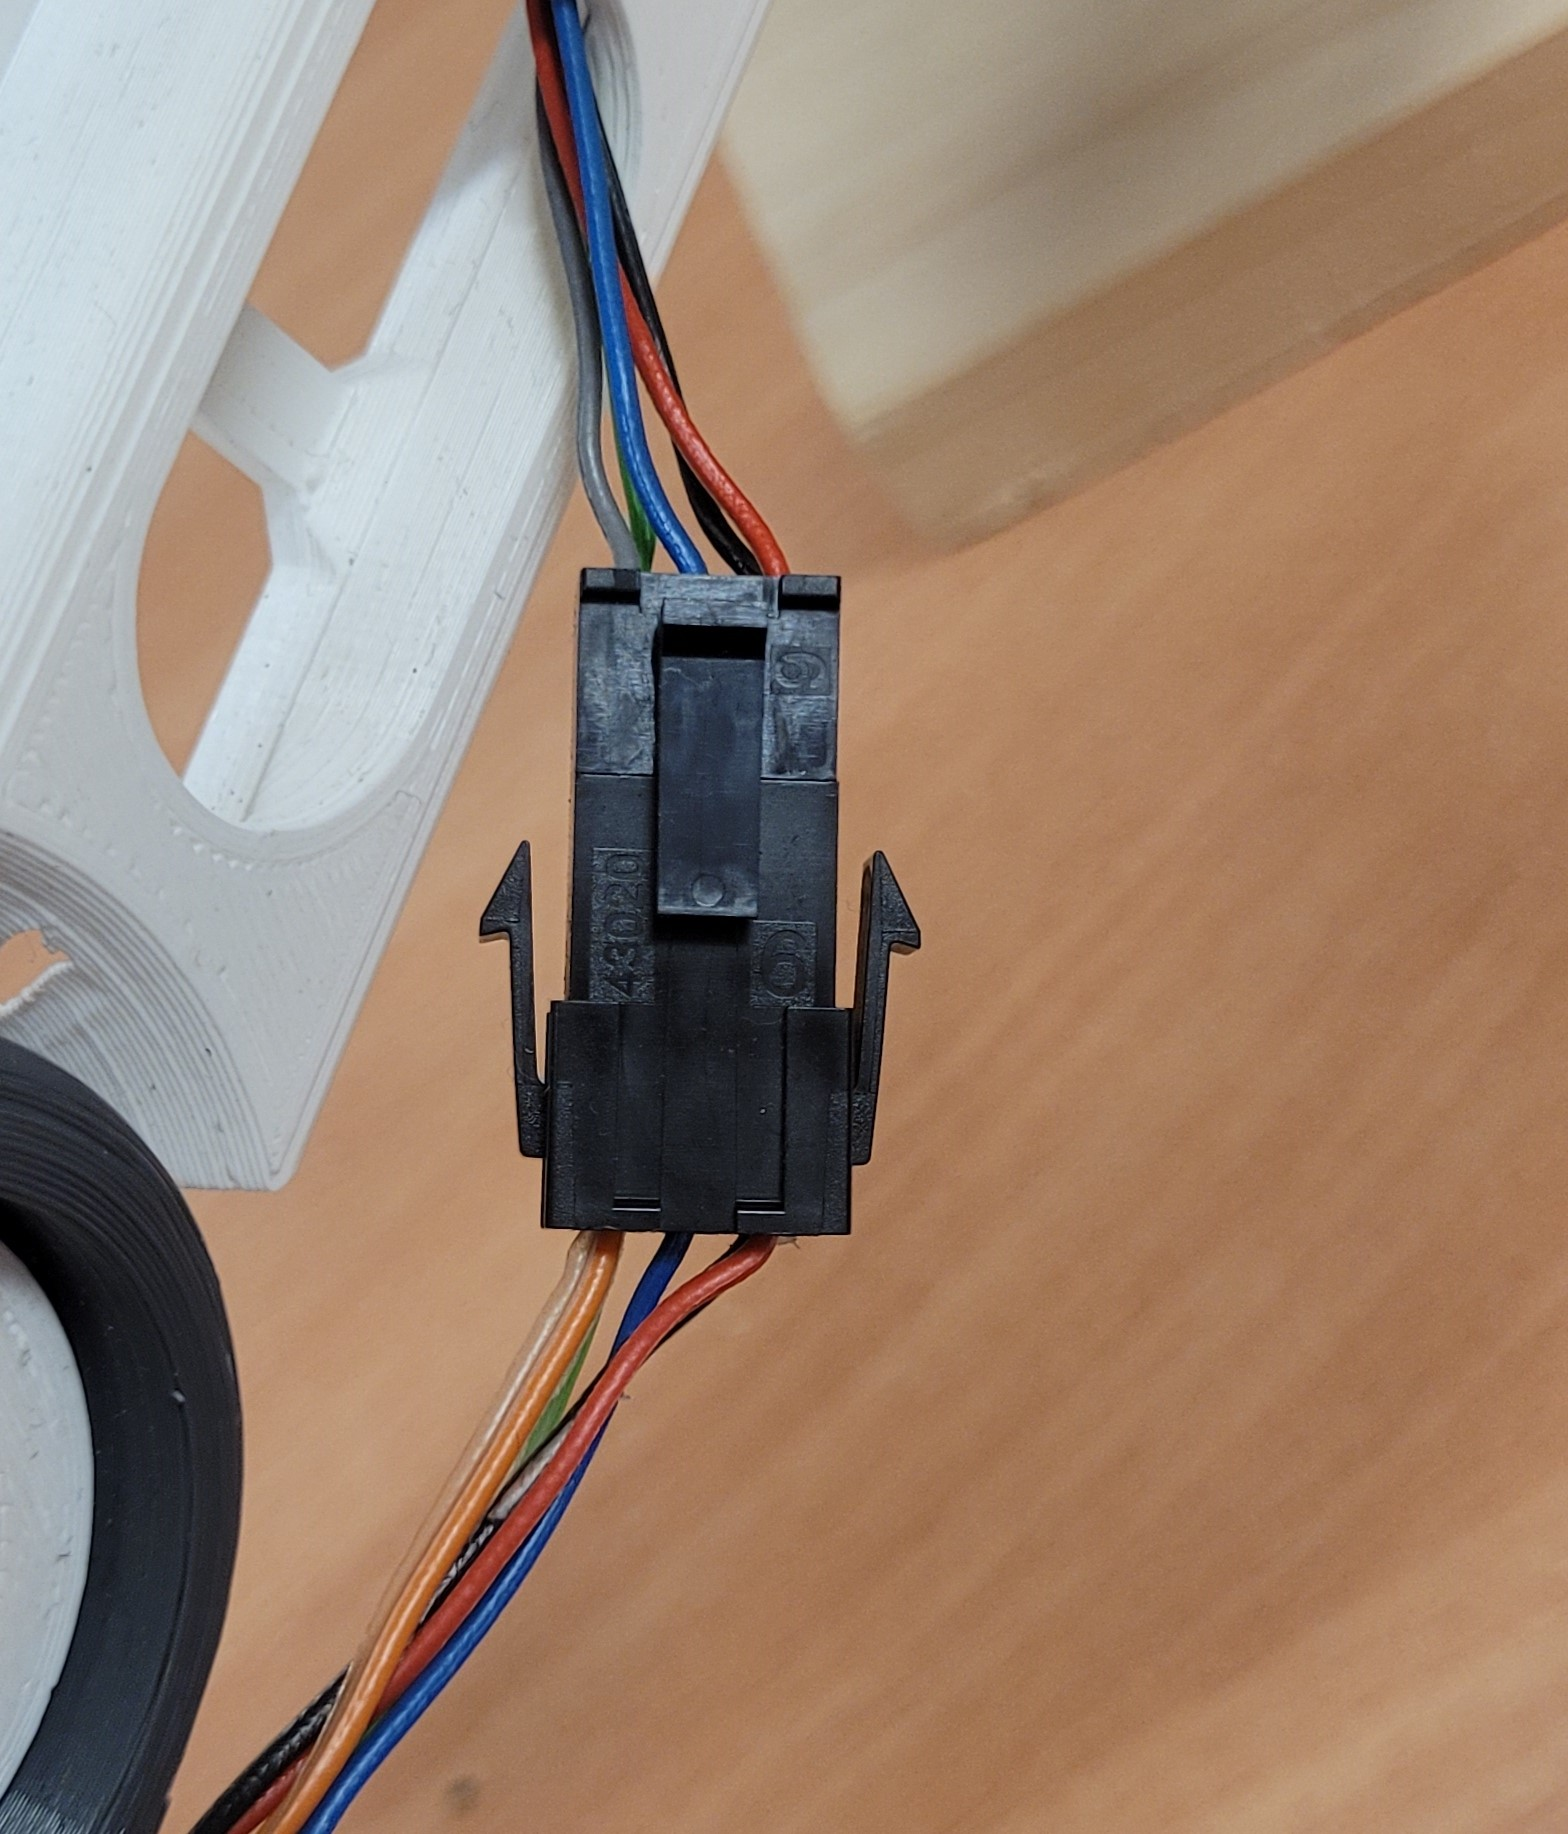
\includegraphics[width=60mm, keepaspectratio]{figures/Csuklo_szog_teszt/molex_valos}
\caption{A negyedik és ötödik kar között található szenzor csatlakozója}
\label{fig:csuklo_csatlakozo}
\end{figure}

\subsection{Mikrovezérlő}
\label{sec:mikrovez_bemut}

Elérkeztünk a mikrovezérlőig, mivel strukturálisan a vezetéken megérkező jeleket érzékelni tudjuk és a mikrovezérlőre csatlakoztatva az ezen futó programmal fel is tudjuk dolgozni. A szakdolgozatomban összeállított telemanipulátorhoz képest itt egy nagyobb komplexitású mikrovezérlőt választottam. Ennek az az oka, hogy a korábban használt eszközben nincs beépített bootloader, a pinek száma lényegesen kisebb és az eszköz memóriája túl kicsi a továbbfejlesztéshez. Ezek alapján döntöttem úgy, hogy a STMicroelectronics által gyártott Nucleo típusú fejlesztő board-ot választom. Az előnye a fejlesztő board-oknak, hogy a gyártó által összeállított tesztelt eszközök. Túlságosan nagy a felhasználhatóságuk, így könnyen pazarló vagy felesleges funkciókat is vásárolhatunk velük, de a prototípus gyártás elengedhetetlen elemei.

\begin{figure}[!ht]
\centering
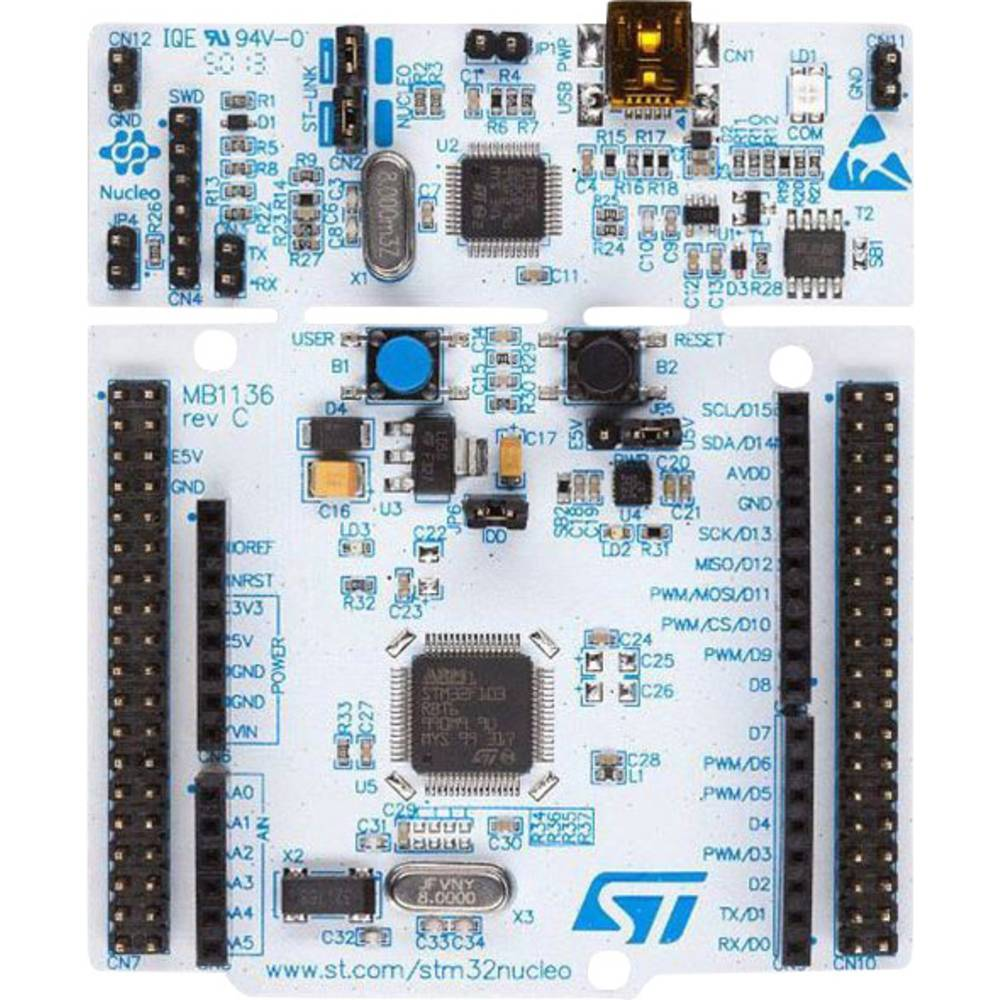
\includegraphics[width=60mm, keepaspectratio]{figures/Csuklo_szog_teszt/mikrovez}
\caption{Az csuklóban található szenzorok működés közben. A kép eredete: \url{https://www.st.com/en/evaluation-tools/nucleo-f401re.html}}
\label{fig:mikrovez}
\end{figure}

Az STM32 Nucleo boardok ezek alapján olyan fejlesztői platformok, amelyek kifejezetten az STMicroelectronics által gyártott STM32 mikroprocesszorokkal való alkalmazásfejlesztés támogatására szolgálnak. A board moduláris felépítésű, lehetővé téve a könnyű kibővítést és testreszabhatóságot. Érdekes előnyük, hogy a diákok körében elterjedt számtalan Arduino Uno és ST Morpho csatlakozók révén a felhasználók könnyen integrálhatnak kiegészítő modulokat, érzékelőket és egyéb hardvereszközöket az adott projekthez. Az STM32 Nucleo boardokat a STM32CubeIDE fejlesztői környezet támogatja, amely egyszerű és hatékony eszköztár a szoftverfejlesztéshez. Az STM32CubeMX grafikus konfigurációs eszköz segítségével könnyedén konfigurálhatók és beállíthatók a perifériák illetve a CubeMonitornak köszönhetően a grafikusan megjeleníthetőek a szenzor adatokhoz tartozó változók. Ennek az eszköznek nagy haszna volt amikor a szenzorok kalibrációját és tesztelését végeztem. A board beépített perifériákkal rendelkezik, mint például érzékelők, LED-ek és gombok, amelyek segítik a prototípusfejlesztést és a beágyazott rendszerek gyors tesztelését. Az én általam használt mikrovezérlő esetében $3[db]$ SPI (XYZ fejezet) kommunikációs port is található, amivel így a továbbfejlesztési lehetőségek száma nagyon megugrik. Az STM32 boardok nagyon jó minőségű és nagy terjedelmű dokumentációval rendelkeznek, beleértve az útmutatókat, példaprogramokat, fórumokat és alkalmazási jegyzeteket. Ennek a hasznosságát nem lehet kellőképpen nyomatékosítani, ugyanis pont a nagy terület lefedés miatt a boradoknál nagyon sok mindenre kell figyelni, hogy a lehető legjobb eredményt érjük el. Az utolsó általános szempont amivel a STM32 Nucleo boardaot vizsgálni lehet, hogy könnyen elérhetők a piacon, számos konfugurációban és a bekerülési költségük összevetve egy cél eszköz gyártásával is elég alacsony.

Az én általam használt STM32 Nucleo board pontos típusa STM32F401RE. A mikrovezérlő az egyik legújabb jelenleg és a háttértára kellő mértékben nagy ahhoz, hogy akár még kijelző vezérlésre is alkalmas legyen amellett, hogy a szenzorokat ugyanazzal a hatásfokkal kezelje, ami a $4[ms]$-os ciklusidő kritériumhoz kell. Az eszköz adatlapja elérhető a mellékletekben (\ref{sec:melleklet}.fejezet) és a részletes specifikáció ismertetése a \ref{sec:STM32_nucleo}, ezek mellett a előző eszközzel való összehasonlítására helyezném a hangsúlyt. A szakdolgozatom során egy STM32F103C8-as típusú mikrovezérlőt használtam. A könnyebb beazonosíthatóság érdekében a processzor típusa helyett a közismertebb nevét használom, ami a Bluepill.

A Bluepill típusú mikrovezérlő kompakt kisméretű, de tág fejlesztési határokat megengedő eszköz. Kis mérete, alacsony bekerülési költsége és alacsonyabb fogyasztása miatt használják. Jellemző felhasználási területe az IoT\footnote{Az Internet of Things az a koncepció, amely szerint különböző eszközök és egységek képesek kommunikálni az interneten, vagy felhőszolgáltatásokon keresztül. Jellemzően adatok gyűjtésére és megosztására használják. Illetve szoros összefüggésben van a "okos"/intelligens funkciók kialakításában.} (Internet of Things), kisebb autonóm rendszerek és adatgyűjtő berendezések. A diploma dolgozatomban bemutatott telemanipulátorhoz használt Nucleo-hoz képest, a Bluepill memóriája lényegesen kisebb, illetve a felhasználható perifériák száma is alacsonyabb. Azonban ez még nem tette szükségessé a lecserélését, inkább a jövőbeli fejlesztési lehetőségek számát korlátozná. A következő táblázatban összegyűjtöttem azt a néhány funkciót, ami miatt a mikrovezérlő cserére döntöttem.

\begin{table}[!h]
\begin{center}
    \begin{tabular}{|c c c|} 
        \hline
        Tulajdonság & STM32 F103C8 & STM32 F401RE  \\ 
        \hline
        Processzor típusa     &  Arm Cortex-M3  &  Arm Cortex-M4  \\
        Flashmemória          & $64[kB]$        & $512[kB]$       \\
        RAM mérete            & $20[kB]$    	& $96[kB]$        \\
        Beépített bootloader  & nincs           & van             \\
        SPI portok száma      & 2               & 3               \\
        \hline
    \end{tabular}
    \caption{STM32-es mikrovezérlő összehasonlítása}
\end{center}
\end{table}

A felsorolt különbségek száma nem sok, de a fejleszthetőséget nagy mértékben megkönnyíti. Az elkészült telemanipulátor jelfeldolgozó rendszer teljesítménye és a tesztelés közben tapasztalt könnyebbségek, illetve a mérete miatt abszolút előrelépésnek, jó döntésnek és sikeres fejlesztésnek állapítom meg a mikrovezérlő cserét.


\subsection{STM32 nucleo}
\label{sec:STM32_nucleo}
%----------------------------------------------------------------------------
Az STM32 mikrovezérlők az STMicroelectronics által gyártott nagyon népszerű és széles körben használt beágyazott rendszerekre szánt eszközök. Az STM32 fejlesztőeszközök a Cortex-M4 processzormaggal rendelkező STM32 mikrovezérlők családjára épülnek. A Cortex-M4 egy ARM architektúrájú processzormag, amelyet beágyazott rendszerekhez terveztek. Nagy teljesítményt és alacsony energiafogyasztást tesz lehetővé.

A NUCLEO-F411RE board egy fejlesztőeszköz az STM32 fejlesztőeszközök palettájáról. Ez a fejlesztői platform az STM32F411RE mikrovezérlőre épül, amely egy Cortex-M4 processzormaggal rendelkező mikrovezérlő. A NUCLEO-F411RE board kiváló mivel komplex fejelsztést tesz lehetővé, és nem kell a mikrovezérlőhöz tartozó hardvert megtervezni. A board számos funkcióval és interfésszel rendelkezik, ideértve digitális és analóg bemeneteket, PWM kimeneteket, UART, I2C, SPI és USB interfészeket, valamint egy ST-Link programozó/debugger egységet. Ez a board könnyen használható és támogatja az alkalmazások gyors prototípus készítésben és tesztelésében.

Az STM32 fejlesztőeszközökön általában kényelmesen használható fejlesztői környezet, például az STM32CubeIDE vagy az STM32CubeMX áll rendelkezésre. Ezek az eszközök számos fejlesztői funkciót és eszközt biztosítanak, például kódszerkesztőt, kódgenerátort, szimulációs lehetőségeket és debugger eszközöket, hogy segítsék a fejlesztőket a hatékony és könnyű fejlesztésben.

\newpage
%----------------------------------------------------------------------------
\section{Összeállított rendszer tesztelése}

A bemutatott komponensekből összeállított rendszer jelen fejlesztési státuszban $7[db]$ GMR szenzorból, $2[db]$ USB csatlakozóból és a STM32-es Nucleo boardból áll. A két USB csatlakozó közül az egyik a STM32-es board tápellátásáért és a mikrovezérlő program felügyeletéért, a másik pedig a adatok továbbításáért felel. A szenzorok a PCB-hez forrasztással lettek rögzítve, csakúgy ahogy a bypass kondenzátor is. A vezetékek a PCB-hez furatokba szintúgy forrasztással lettek bekötve. A MOLEX csatlakozókba a vezetékek alakkal zárással lettek rögzítve, illetve a mikrovezérlőre a SSC kommunikációs protokolhoz (\ref{sec:ssc_kom} fejezet) tartozó $SCK$ és $DATA$ vezeték a szenzortápok pozitív és negatív pólusával egyetemben funkciónként közösítve lettek. Minden a mikrovezérlőre közvetlenül csatlakozó vezeték dupont\footnote{Fejlesztésnél előszeretettel használt pin-re könnyen rögzíthető akárcsak 1-1 vezeték rögzítésére alkalmas csatlakozó.} csatlakozóval lett a megfelelő helyre kötve.

\begin{figure}[!ht]
\centering
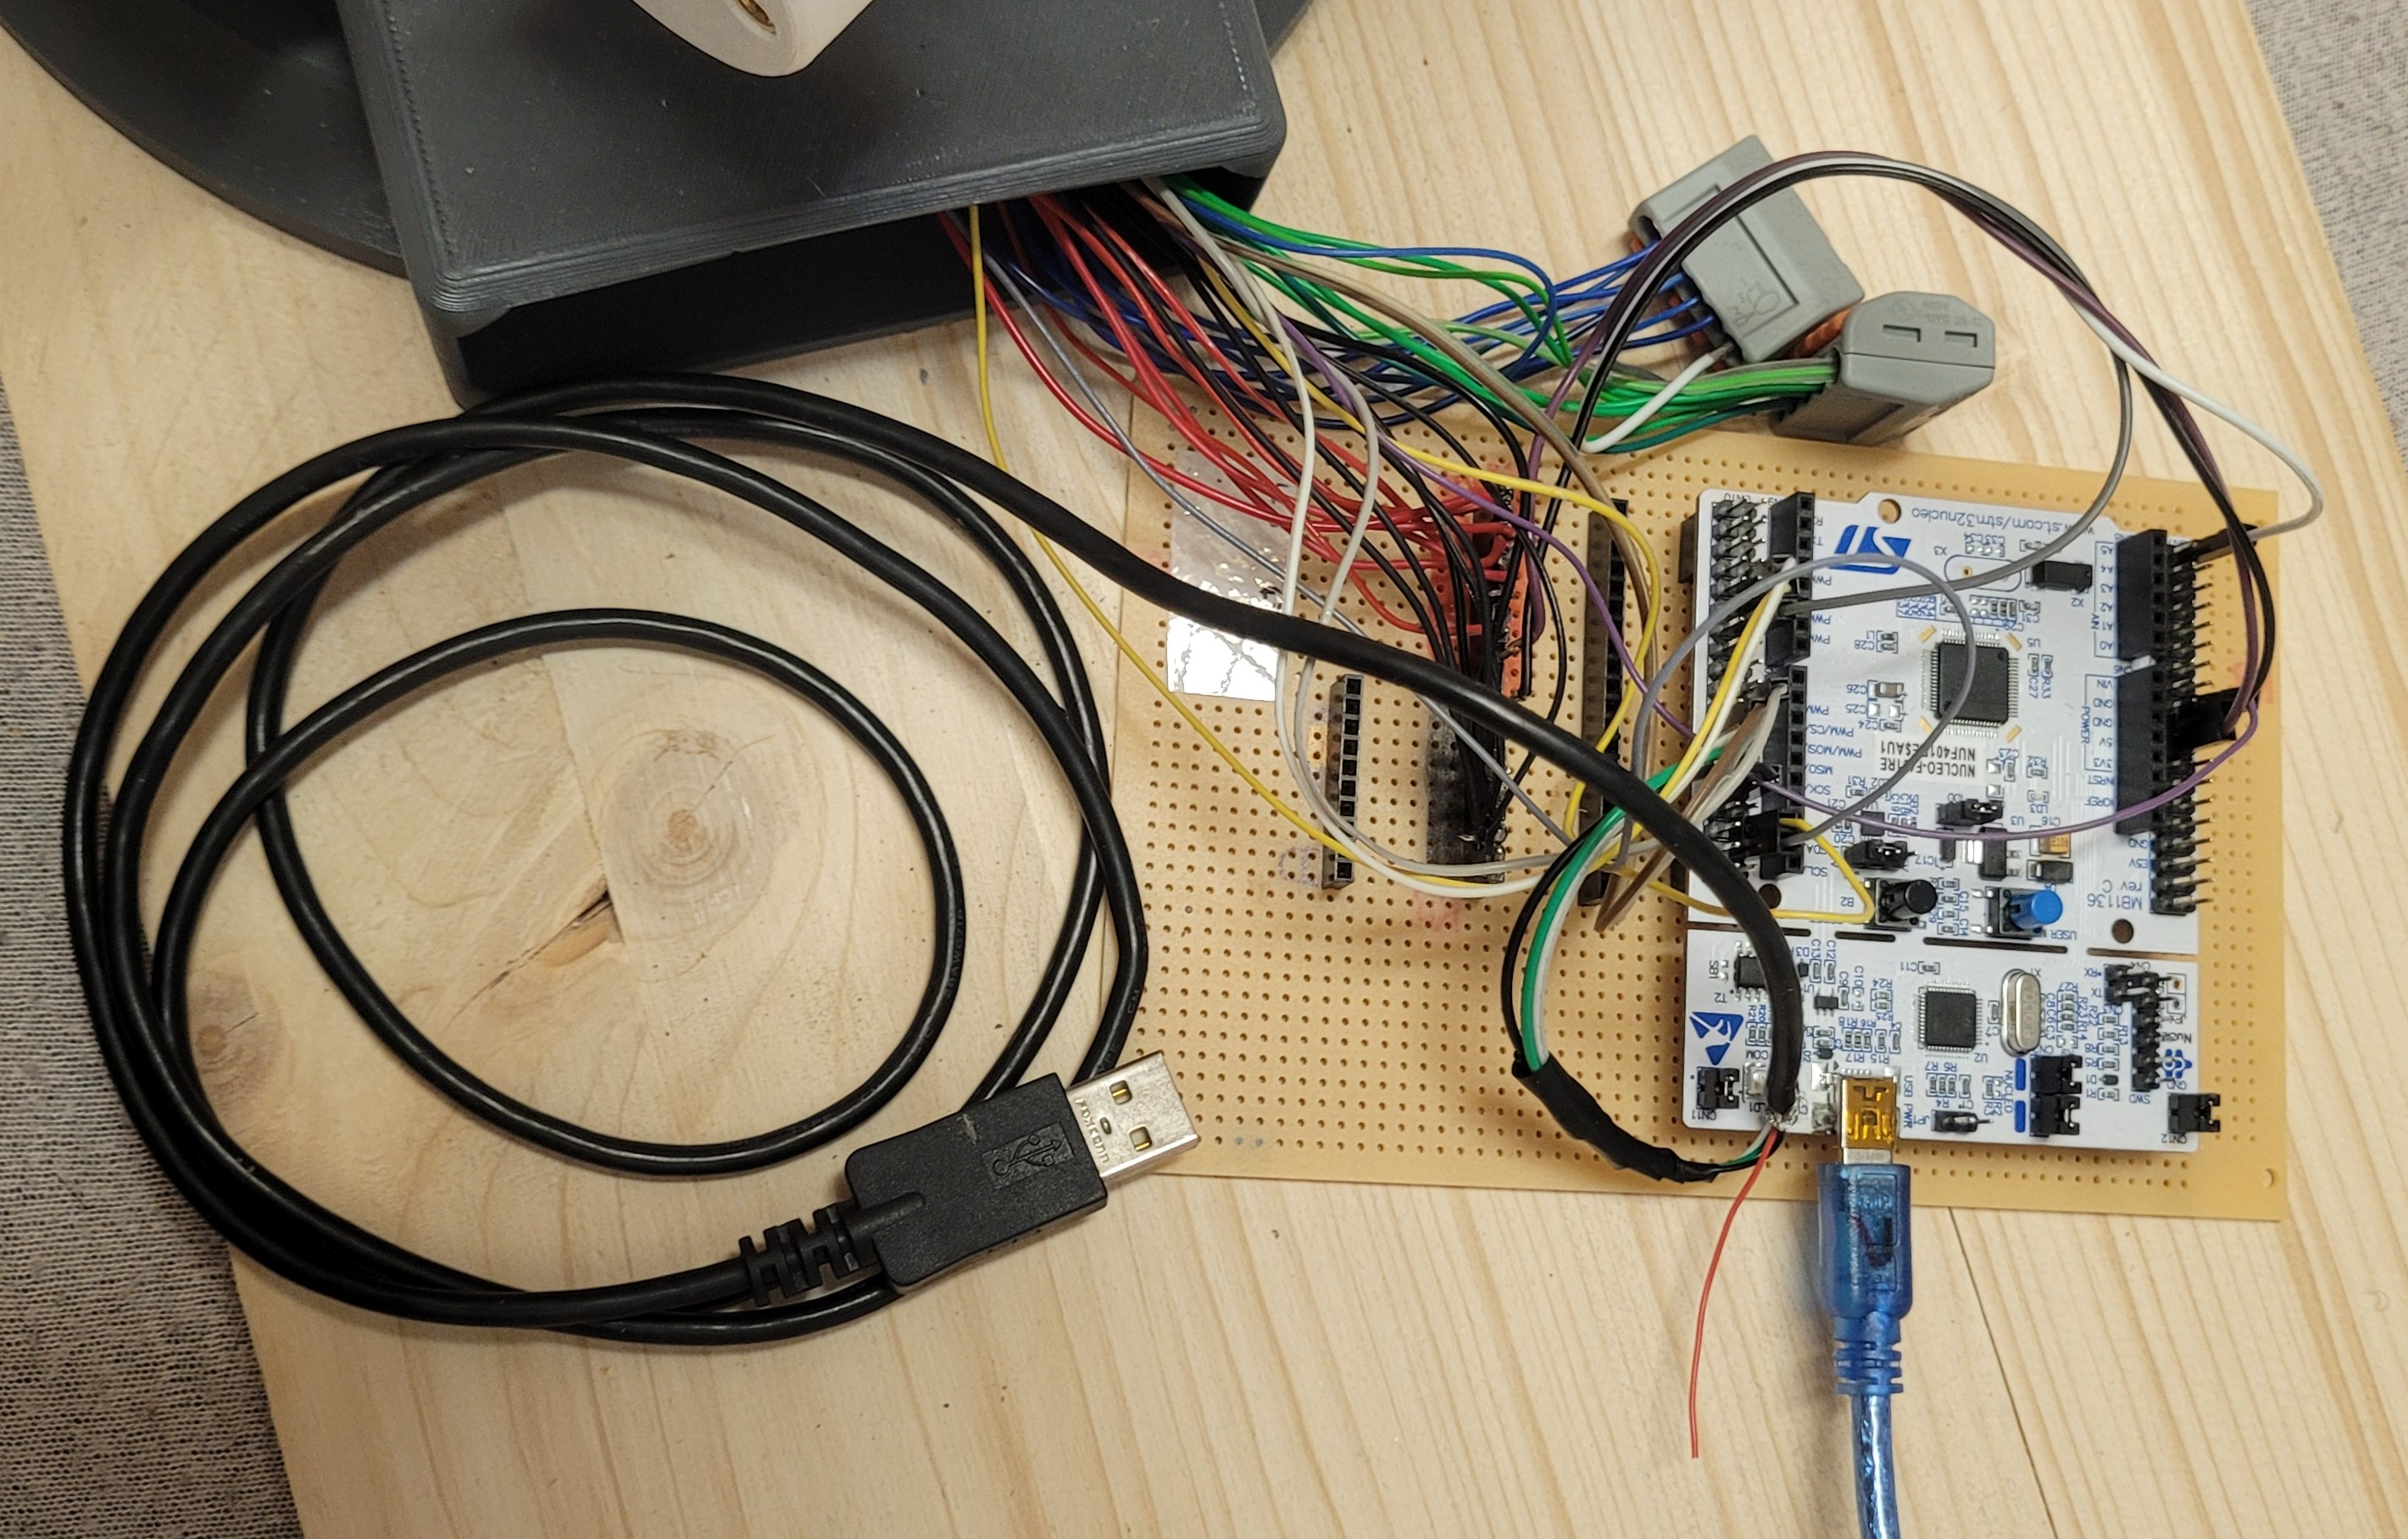
\includegraphics[width=100mm, keepaspectratio]{figures/Csuklo_szog_teszt/mikrovez_2}
\caption{Az összeállított rendszer}
\label{fig:szummarendszer}
\end{figure}


\newpage
\subsection{GMR szenzorok tesztelése}

A következő képeken dokumentáltam a szenzorok egyenkénti működését.

\begin{figure}[!ht]
\centering
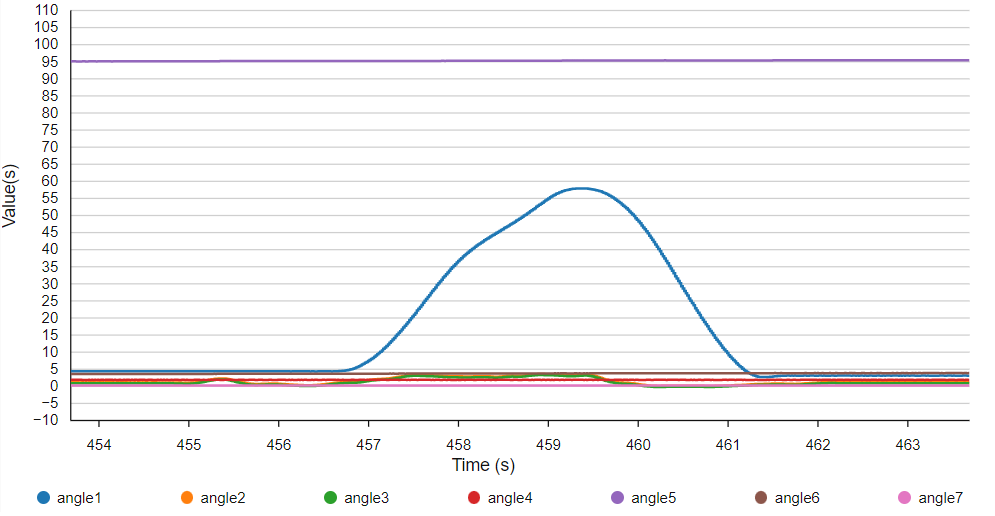
\includegraphics[width=100mm, keepaspectratio]{figures/Csuklo_szog_teszt/1}
\caption{Az első csuklóban található szenzor tesztje}
\label{fig:csuklo_teszt_1}
\end{figure}

\begin{figure}[!ht]
\centering
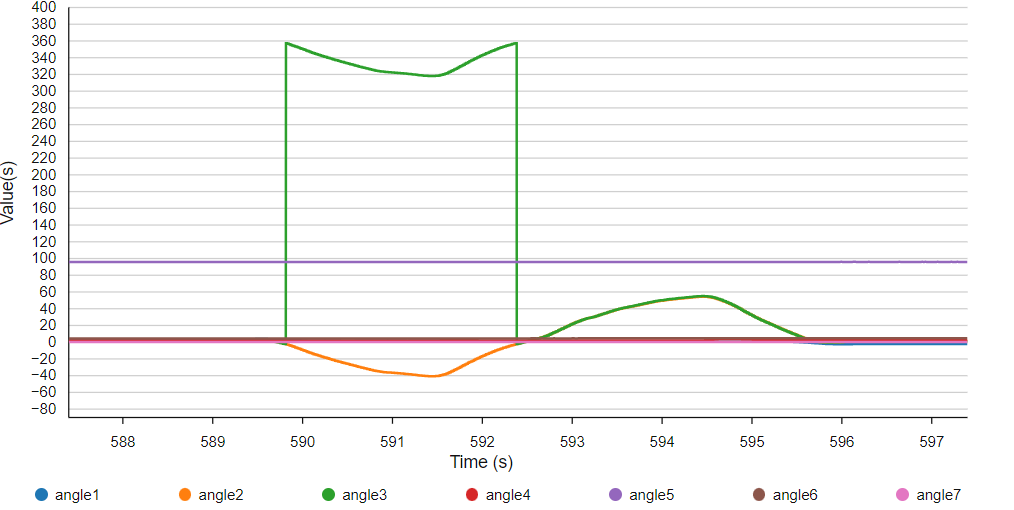
\includegraphics[width=100mm, keepaspectratio]{figures/Csuklo_szog_teszt/2_3}
\caption{Az második csuklóban található szenzor tesztje}
\label{fig:csuklo_teszt_2_3}
\end{figure}

\begin{figure}[!ht]
\centering
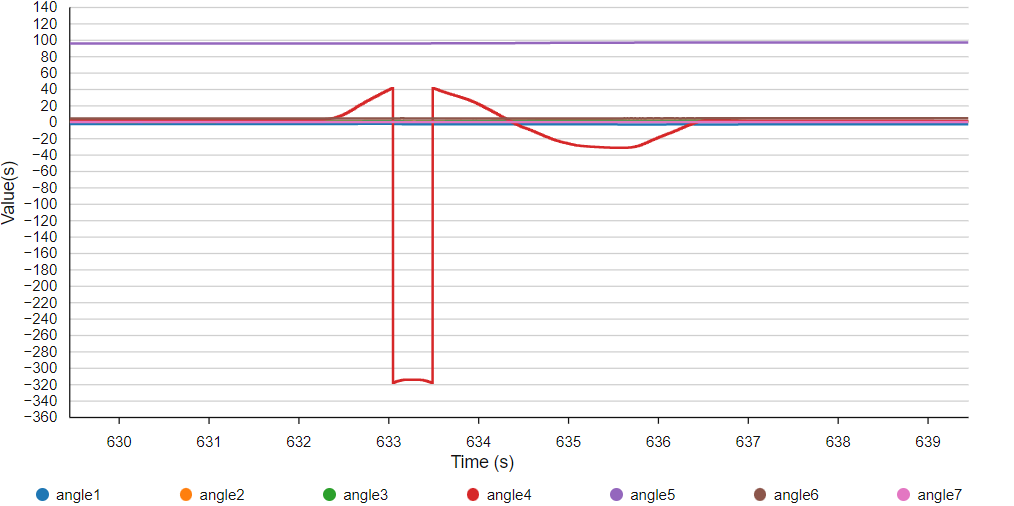
\includegraphics[width=100mm, keepaspectratio]{figures/Csuklo_szog_teszt/4}
\caption{Az harmadik csuklóban található szenzor tesztje}
\label{fig:csuklo_teszt_4}
\end{figure}

\begin{figure}[!ht]
\centering
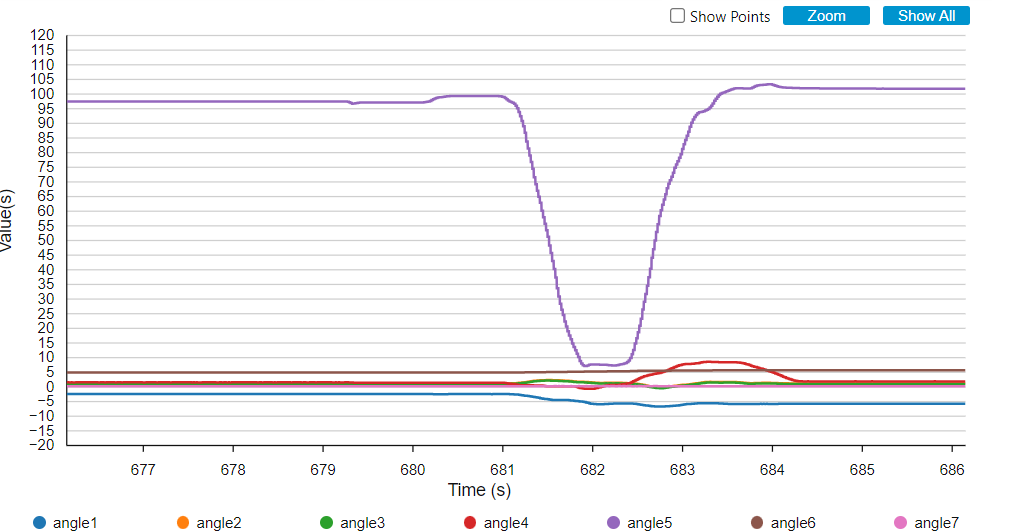
\includegraphics[width=100mm, keepaspectratio]{figures/Csuklo_szog_teszt/5}
\caption{Az negyedik csuklóban található szenzor tesztje}
\label{fig:csuklo_teszt_5}
\end{figure}

\begin{figure}[!ht]
\centering
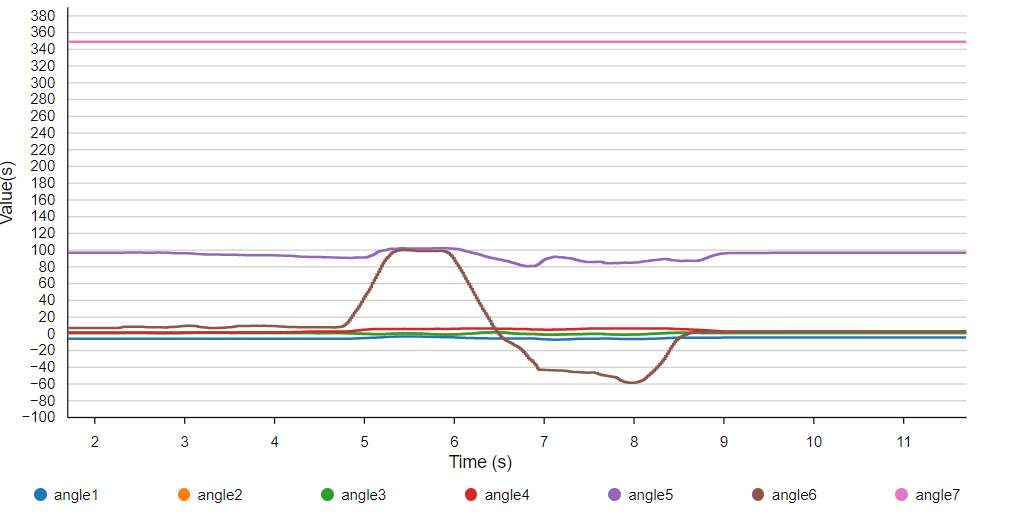
\includegraphics[width=100mm, keepaspectratio]{figures/Csuklo_szog_teszt/6}
\caption{Az ötödik csuklóban található szenzor tesztje}
\label{fig:csuklo_teszt_6}
\end{figure}

\begin{figure}[!ht]
\centering
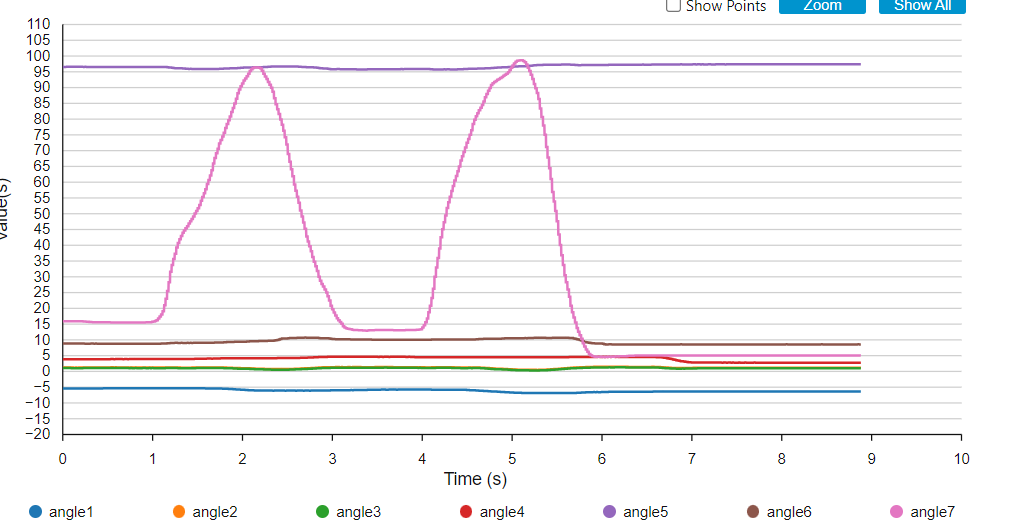
\includegraphics[width=100mm, keepaspectratio]{figures/Csuklo_szog_teszt/7}
\caption{Az hatodik csuklóban található szenzor tesztje}
\label{fig:csuklo_teszt_7}
\end{figure}

\begin{figure}[!ht]
\centering
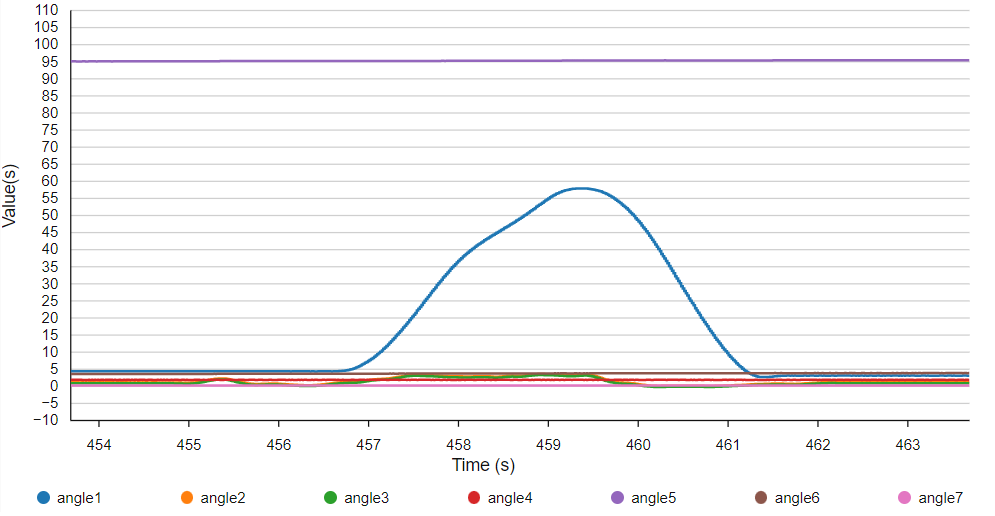
\includegraphics[width=100mm, keepaspectratio]{figures/Csuklo_szog_teszt/1}
\caption{Az első csuklóban}
\label{fig:csuklo_teszt_1}
\end{figure}

Minden szenzor tökéletesen működik. A csukló szöge néhol azért léphetik át a negatív félsíkre, mert a szenzor üzembe helyezés pillanatában, még az offeszetelés nem volt tökéletesen implementálva. Az offszetelést némiképpen pontosabban is lehetne végezni, de ez még a robot használatának szempontjából nem fatális hiba.


\subsection{Vezeték ellenállás mérése}

A vezeték hosszának figyelembe vételével azért szerettem volna foglalkozni, mert az egyik tovább fejlesztési lehetőség amit szeretnék megvalósítani vezeték nélkül kötné össze a telemanipulátort a robot vezérlővel (XYZ fejezet). A vezeték nélküli kommunikáció, ugyan a mikrovezérlő után valósulna meg és nem a szenzor és a közte. Úgy vélem meggyőződni, hogy mekkora lehet a maximális vezeték amit használatok a telemanipulátoron mindenképpen fontos, mert így a impedanciák és interferenciákból fakadó hibákat, illetve továbbfejlesztés esetében figyelembe tudom venni.


%----------------------------------------------------------------------------
%----------------------------------------------------------------------------
